\documentclass[conference]{IEEEtran}
\IEEEoverridecommandlockouts

\usepackage{cite}
\usepackage{amsmath,amssymb,amsfonts}
\usepackage{booktabs}
\usepackage{balance}
\usepackage{graphicx}
\usepackage{microtype}
\usepackage{url}
\usepackage{xcolor}
\usepackage[hidelinks]{hyperref}

\def\BibTeX{{\rm B\kern-.05em{\sc i\kern-.025em b}\kern-.08em
    T\kern-.1667em\lower.7ex\hbox{E}\kern-.125emX}}
\newcommand{\vect}[1]{\boldsymbol{#1}}

\begin{document}

\title{Configurable Signed-Distance-Field-Aware Planning and Whole-Body Model
Predictive Control for Heterogeneous Mobile Manipulators}

\author{\IEEEauthorblockN{Xiaochen Miao}
\IEEEauthorblockA{Technical University of Munich\\
Munich, Germany\\
xiaochen.miao@tum.de}}

\maketitle

\begin{abstract}
Collision avoidance with whole-body model predictive control (WB-MPC) is
challenging because mobile manipulators must coordinate base and arm motion
under platform-specific kinematic and mobility constraints.  This work presents
a configurable collision-aware framework that combines Open Motion Planning
Library (OMPL) reference planning with WB-MPC.  A shared Euclidean signed
distance field (ESDF) provides two collision-avoidance layers: OMPL generates a
collision-checked path, and WB-MPC maintains clearance while tracking it.  On a
nonholonomic Stretch and a holonomic mobile UR10, the framework achieves 16.6-
and 18.5-mm end-effector reference RMSE with positive executed-state collision
margins.  The mobile UR10 also requires less OCP solve time, showing the effect
of base mobility on optimization difficulty.  Deployment on a physical Stretch
demonstrates end-to-end operation with real localization, mapping, and command
execution.
\end{abstract}

\begin{IEEEkeywords}
mobile manipulation, model predictive control, configurable robotics, motion
planning, Euclidean signed distance field, ROS~2
\end{IEEEkeywords}

\section{Introduction}

Mobile manipulators enlarge an arm's workspace through coordinated base motion,
but a controller designed for one platform is often difficult to reuse on
another.  Robots can have different kinematics, base types, collision models,
and command interfaces.  Stretch combines a differential-drive base, lift,
telescopic arm, and wrist~\cite{kemp2022stretch}; the mobile UR10 considered
here combines a six-axis arm with a holonomic planar base.  A reusable framework
must support both without changing its core planning and control algorithms.

Global planning and receding-horizon control offer complementary capabilities.
A sampling-based planner can find a collision-free route over a large
workspace, but its geometric path does not account for tracking error, coupled
dynamics, or input limits.  WB-MPC handles these effects locally, but its finite
horizon is a poor substitute for global routing.  The proposed architecture
therefore uses OMPL to generate an ESDF-validated reference and WB-MPC to track
it while an ESDF collision cost reshapes the predicted trajectory.  The shared
ESDF keeps both collision-avoidance layers geometrically consistent.

Portability here does not mean using an identical model for every robot.
Instead, each URDF/YAML profile is used to generate a robot-specific OCP.  The
profile determines the controlled joints and task frames, base dynamics,
bounds, collision spheres, horizon, and cost weights.  The generated solver
therefore changes with the robot, while the planner, MPC construction, and
execution code remain shared.  At runtime, a platform adapter maps the common
state and trajectory interfaces to the corresponding robot driver.  The
current Stretch adapter additionally performs state fusion, execution
preflight, and deadline-based command holds.

Accordingly, this report asks: \emph{Can an ESDF-aware OMPL--WB-MPC pipeline be
configured for mobile manipulators with different arm dimensions and base
kinematics, while retaining a consistent collision model and explicit hardware
interfaces?}  The main contributions are:
\begin{itemize}
  \item a YAML/URDF-parameterized whole-body MPC formulation that selects state
        and input dimensions, kinematics, bounds, collision geometry, and base
        dynamics for each robot;
  \item a two-layer collision-avoidance design in which OMPL performs
        ESDF-based path validation and WB-MPC applies a differentiable ESDF
        collision cost along the prediction horizon;
  \item a cross-platform evaluation on nonholonomic Stretch and holonomic
        mobile-UR10 models, including tracking, clearance, solver-tail, and
        runtime-decomposition results; and
  \item a physical Stretch demonstration integrating Spectacular AI
        SLAM and an nvblox-derived ESDF with the planning--control loop.
\end{itemize}

The simulation supports a controlled quantitative comparison of the two robot models.
A complementary Stretch real experiment evaluates transfer to physical sensing and
actuation.

\section{Related Work}

\subsection{Mobile-Manipulator Planning and Control Paradigms}

Conventional mobile-manipulation pipelines often decompose a task into base
navigation followed by arm manipulation.  This separation reduces the
dimension of each planning problem and permits reuse of established navigation
and manipulator controllers, but it discards base--arm redundancy and can
produce conservative or suboptimal whole-body motion when the two subsystems
must cooperate in constrained environments.

Kinematic whole-body control instead treats the base and arm as one redundant
chain and resolves task-space commands at the velocity level.  Seraji extended
configuration control to holonomic and nonholonomic mobile manipulators,
incorporating base constraints and auxiliary tasks in a unified kinematic
formulation~\cite{seraji1998unified}.  De Luca \emph{et al.} further considered
nonholonomic mobile manipulators with steering wheels and used task-Jacobian
null-space optimization and feedback linearization to determine otherwise
unspecified steering motions~\cite{deluca2010kinematic}.  These approaches are
computationally efficient, but primarily resolve instantaneous kinematic tasks
rather than predicting the coupled system evolution over a finite horizon.

Sampling-based predictive control provides another route to coupled and
reactive motion.  MPPI updates a nominal control sequence from the costs of
sampled trajectory rollouts and can therefore accommodate complex or
nonsmooth objectives without differentiating the complete cost.  STORM
demonstrated GPU-parallel sampling MPC for a 7-DoF manipulator
~\cite{bhardwaj2022storm}, while Pezzato \emph{et al.} extended GPU-parallel
rollouts to navigation, contact-rich manipulation, and high-dimensional
whole-body control~\cite{pezzato2025sampling}.  RAMP combined an MPPI variant
with an implicit configuration-space SDF for reactive obstacle avoidance
~\cite{vasilopoulos2023ramp}.  Such sampling-based methods are flexible, but
whole-body collision avoidance requires rollout costs across samples, horizon
nodes, and represented robot bodies, commonly motivating substantial GPU
parallelism.  The present framework instead exploits ESDF gradients within a
gradient-based model predictive controller.

\subsection{Whole-Body Model Predictive Control}

Whole-body MPC extends coordinated control beyond instantaneous kinematic
resolution by optimizing the coupled base--arm evolution over a finite
horizon.  It repeatedly solves a finite-horizon problem from the latest state
and executes only the first portion of the optimized sequence, allowing
tracking, effort, smoothness, bounds, and collision terms to be treated
together.

Whole-body MPC also couples manipulation with platform stability.  Minniti
\emph{et al.} formulated manipulation, balancing, and interaction as one
finite-horizon optimal-control problem for an inherently unstable
ball-balancing mobile manipulator.  Their formulation predicts how
end-effector tracking and contact-force decisions affect the future balance of
the system, and was validated in hardware pose-tracking and door-opening
experiments~\cite{minniti2019wholebody}.  This work establishes the value of
jointly optimizing platform and manipulator behavior, but focuses on dynamic
stabilization of a ballbot.  The present work applies a unified predictive
structure to kinematically different wheeled mobile manipulators.  Enabling
online whole-body collision avoidance within this structure additionally
requires an environmental representation that can be queried efficiently at
many prediction states, motivating the distance-field methods discussed next.

\subsection{Distance-Field-Based Collision Avoidance}

Conventional collision checking evaluates the geometric relationship between
robot links and environmental obstacles explicitly. Depending on the
environment representation, this may involve repeated collision or distance
queries between robot meshes or collision primitives and individual obstacle
geometries~\cite{pan2012fcl}. Such pairwise geometric queries can become computationally
expensive when they are repeatedly evaluated for multiple robot links and
prediction states within an online optimization loop.

Distance-field representations instead encode obstacle proximity independently
of the robot geometry.  ESDFs provide continuous clearance values and local
spatial gradients, making them suitable for optimization-based motion
generation.  Voxblox demonstrated incremental ESDF construction from a TSDF
for onboard planning~\cite{oleynikova2017voxblox}, while nvblox accelerates
dense incremental mapping on a GPU~\cite{millane2023nvblox}.

Distance fields have consequently been integrated into reactive
motion-generation systems.  Gaertner \emph{et al.} used a dynamically generated
ESDF for static collision checking and moving-obstacle models for dynamic
scenes within a legged-robot MPC~\cite{gaertner2021collisionfree}.  Chiu \emph{et al.} incorporated
an environment SDF into whole-body MPC and demonstrated collision-aware
locomotion and manipulation while caching distance and gradient information to
reduce environment-query overhead~\cite{chiu2022collisionfree}.  Both studies
were validated on quadrupedal robot platforms: the former focused on legged
locomotion, whereas the latter extended collision-aware MPC to legged mobile
manipulation.  They demonstrate the benefits of distance fields for reactive
collision avoidance, but do not directly address a shared whole-body planning
and control framework configurable for wheeled mobile manipulators with
different arm dimensions and base kinematics.

\section{Method}

\subsection{Robot-Parameterized Control Framework}

The framework accepts a URDF and a composed YAML robot profile.  The URDF
defines the joints and links, kinematic tree, frame transforms, joint types,
and arm joint-position limits.  The profile selects the controller joint
ordering and task frames from that model, and supplies controller-level choices
not encoded by the URDF: the base dynamics, base workspace and velocity/input
bounds, collision-sphere approximation, horizon, and cost weights.  Pinocchio
and CasADi combine these inputs to construct a robot-dimensioned symbolic OCP,
from which acados generates a robot-specific solver.
Changing the arm dimension, base dynamics, or number of collision spheres
regenerates the solver but does not change the construction procedure.

At runtime, a control goal is converted into a reference horizon,
the ESDF supplies local obstacle information, and the generated solver jointly
optimizes base and arm motion.  A platform adapter then converts the optimized
trajectory into robot commands.  Figure~\ref{fig:system-overview} summarizes
both offline robot specialization and the online feedback-control path.

\begin{figure*}[t]
  \centering
  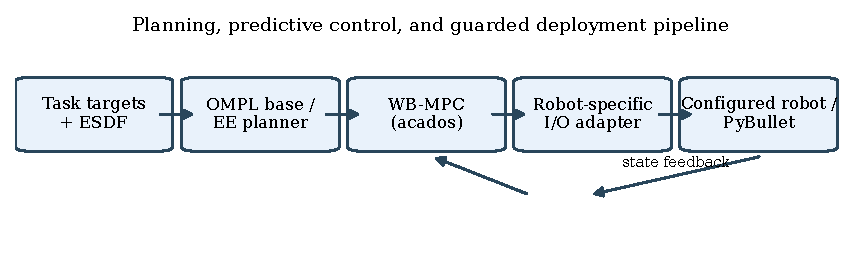
\includegraphics[width=\textwidth]{figures/system_overview.pdf}
  \caption{Robot-parameterized solver generation and online control flow.  A
  URDF and YAML profile specialize the generated solver; control targets and
  ESDF data then enter the shared WB-MPC path before platform-specific command
  mapping.}
  \label{fig:system-overview}
\end{figure*}

The following subsections define the dynamics, ESDF collision model, OCP, and
task-conditioned reference generation used in this pipeline.

\subsection{Model Predictive Control}

\subsubsection{Robot-Parameterized Dynamics}

Each robot profile selects the base dynamics branch: an omnidirectional base
uses a planar double-integrator model, whereas a nonholonomic base can use the
embedded no-slip dynamics derived below.  The URDF specializes the arm
dimension and kinematics, and all arm joints use acceleration-controlled
double-integrator dynamics.

For a robot with $n_a$ independent arm coordinates, the optimizer constructs
\begin{equation}
\vect{q}=\begin{bmatrix}x&y&\theta&\vect{q}_a^{\top}\end{bmatrix}^{\!\top},
\quad
\vect{x}=\begin{bmatrix}\vect{q}^{\top}&\vect{v}^{\top}\end{bmatrix}^{\!\top},
\label{eq:q}
\end{equation}
The corresponding continuous-time state equation is written generically as
\begin{equation}
\dot{\vect{x}}=f(\vect{x},\vect{u})
=\begin{bmatrix}
\dot{\vect{q}}^{\top}&\dot{\vect{v}}^{\top}
\end{bmatrix}^{\!\top},
\label{eq:state-dynamics}
\end{equation}
where $(x,y,\theta)$ is the map-frame planar base pose.  Let $n_q$, $n_u$, and
$n_x$ denote the dimensions of the generalized-coordinate vector, optimizer
input, and state vector, respectively.  The planar base contributes three
coordinates, while the arm contributes $n_a$ independent coordinates; hence,
$n_q=3+n_a$.  Because the optimizer assigns one acceleration input to each
generalized coordinate, $n_u=n_q$.  The state stacks generalized positions and
velocities, giving $n_x=2n_q$.  These dimensions describe the internal
optimization model rather than the number of physical actuators.  Joint names,
bounds, link frames, tool and base links, collision primitives, and URDF are
read from the selected robot profile.

For an omnidirectional base, every coordinate follows the common
double-integrator model $\dot{\vect{q}}=\vect{v}$,
$\dot{\vect{v}}=\vect{u}$, and therefore
\begin{equation}
\dot{\vect{x}}_{\mathrm{omni}}
=\begin{bmatrix}\vect{v}^{\top}&\vect{u}^{\top}\end{bmatrix}^{\!\top}.
\label{eq:omni-state-dynamics}
\end{equation}
For a nonholonomic base in dynamics mode, the same
public world-frame state $[v_x,v_y,\omega]$ is retained, but the base part is
replaced by a no-slip model.  Its forward and lateral components are
\begin{align}
v_f &= \cos\theta\,v_x+\sin\theta\,v_y, \\
v_{\mathrm{lat}} &= -\sin\theta\,v_x+\cos\theta\,v_y=0. \label{eq:no-slip}
\end{align}
The first two world-frame acceleration variables are similarly projected to
$a_f=\cos\theta\,a_x+\sin\theta\,a_y$.  The embedded base dynamics are
\begin{align}
\dot{x}&=v_f\cos\theta,&
\dot{y}&=v_f\sin\theta,&
\dot{\theta}&=\omega,\\
\dot{v}_x&=a_f\cos\theta-\omega v_f\sin\theta,\\
\dot{v}_y&=a_f\sin\theta+\omega v_f\cos\theta,\\
\dot{\omega}&=\alpha. \label{eq:unicycle}
\end{align}
These equations define the two base-dynamics branches selected by the robot
profile.

\subsubsection{ESDF Collision Avoidance}

The environment representation is independent of the robot model.  Each robot
profile instead attaches a set of collision spheres to selected links.  Given
configuration $\vect{q}_k$, forward kinematics determines the center
$\vect{c}_j(\vect{q}_k)$ of sphere $j$.  Define the configuration-dependent
clearance as $d_j(\vect{q})\triangleq d(\vect{c}_j(\vect{q}))$, where the ESDF
returns both the signed distance and its spatial gradient.

The exported ESDF is sampled on a regular three-dimensional grid.  A query
point is first located within a grid cell.  The implementation then uses its
relative position along the three coordinate axes to trilinearly interpolate
both the distance and the stored gradient from the cell's eight corners.  The
resulting signed distance and spatial gradient are denoted by
$\widehat d(\vect{c})$ and $\widehat{\vect{n}}(\vect{c})$, respectively.  Under
the conservative validity policy used in the experiments, a query is accepted
only if it lies inside the grid and all eight interpolation corners are marked
valid.  The interpolation supplies a continuous local distance--gradient pair
to the MPC update.

Because the gridded ESDF is queried outside the generated acados solver, its
local values are updated from the warm-start trajectory before every MPC
solve.  At shooting node $k$, the first-order Taylor model around the sphere
center $\vect{c}_j(\bar{\vect{q}}_k)$ is
\begin{equation}
\begin{aligned}
\widetilde d_{j,k}(\vect{q})={}&
\widehat d\!\left(\vect{c}_j(\bar{\vect{q}}_k)\right)\\
&+\widehat{\vect{n}}\!\left(\vect{c}_j(\bar{\vect{q}}_k)\right)^{\top}
\left(\vect{c}_j(\vect{q})-\vect{c}_j(\bar{\vect{q}}_k)\right).
\end{aligned}
\label{eq:esdf-linearization}
\end{equation}
Thus, the solver retains the robot-specific forward-kinematics expression
$\vect{c}_j(\vect{q})$ but replaces the external map query with a local affine
distance-field model.  The way this model produces a gradient with respect to
the robot coordinates can be seen directly from its differential.  Define the
point Jacobian
$J_{\vect{c}_j}(\vect{q})\triangleq
\partial\vect{c}_j(\vect{q})/\partial\vect{q}$.  A small configuration change
$\delta\vect{q}$ moves the sphere center by
\begin{equation}
\delta\vect{c}_j=J_{\vect{c}_j}(\vect{q})\,\delta\vect{q}.
\end{equation}
The ESDF distance and gradient evaluated at the warm-start center remain
constant during one solve.  Differentiating Eq.~\eqref{eq:esdf-linearization}
therefore gives
\begin{equation}
\begin{aligned}
\delta\widetilde d_{j,k}
&=\widehat{\vect{n}}\!\left(\vect{c}_j(\bar{\vect{q}}_k)\right)^{\top}
  \delta\vect{c}_j\\
&=\widehat{\vect{n}}\!\left(\vect{c}_j(\bar{\vect{q}}_k)\right)^{\top}
  J_{\vect{c}_j}(\vect{q})\,\delta\vect{q}.
\end{aligned}
\end{equation}
By the gradient definition
$\delta\widetilde d_{j,k}=(\nabla_{\vect{q}}\widetilde
d_{j,k})^{\top}\delta\vect{q}$, comparison of the two expressions yields
\begin{equation}
\nabla_{\vect{q}}\widetilde d_{j,k}(\vect{q})
=J_{\vect{c}_j}(\vect{q})^{\top}
 \widehat{\vect{n}}\!\left(\vect{c}_j(\bar{\vect{q}}_k)\right).
\label{eq:linearized-esdf-gradient}
\end{equation}
In physical terms, each column of the point Jacobian describes how one robot
coordinate moves the sphere center, while its dot product with
$\widehat{\vect{n}}(\vect{c}_j(\bar{\vect{q}}_k))$ measures how strongly that
motion increases or decreases the local obstacle distance.  The code does not
explicitly construct this matrix product or query a new ESDF gradient inside
acados.  CasADi obtains it by automatically differentiating the local distance
model; the interpolated gradient remains fixed until the next MPC update.

For sphere radius $r_j$ and configured safety distance $d_s$, the geometric
margin at prediction node $k$ is
\begin{equation}
m_{j,k}=d\!\left(\vect{c}_j(\vect{q}_k)\right)-r_j-d_s.
\label{eq:margin}
\end{equation}
Inside the solver, $d$ is replaced by the Taylor model in
Eq.~\eqref{eq:esdf-linearization}, giving
$\widetilde m_{j,k}=\widetilde d_{j,k}(\vect{q}_k)-r_j-d_s$.  The collision
condition is implemented as a soft cost rather than a hard inequality
constraint.  Specifically, the implementation uses a smooth relaxation of the
hinge violation $\max(0,-m)$ and then squares it:
\begin{align}
v_{\varepsilon}(m)
  &=\frac{1}{2}\!\left(\sqrt{m^2+\varepsilon^2}-m\right),\\
\phi(m)
  &=\frac{1}{2}\mu\,v_{\varepsilon}(m)^2
   =\frac{\mu}{8}\!\left(\sqrt{m^2+\varepsilon^2}-m\right)^2.
\label{eq:smooth-hinge}
\end{align}
As $\varepsilon\rightarrow0$, $\phi(m)$ converges to
$\tfrac{1}{2}\mu\max(0,-m)^2$.  The total collision cost over the prediction
horizon is then
\begin{equation}
J_{\mathrm{obs}}=\sum_{k=0}^{N-1}\sum_{j=1}^{n_c}
\phi(\widetilde m_{j,k}),
\label{eq:sdf-cost}
\end{equation}
where $n_c$ denotes the number of collision spheres attached to the robot.
The Stretch and mobile-UR10 profiles supply 34 and 93 link-attached spheres,
respectively.  At every MPC update, ESDF values and gradients are queried along
the warm-start trajectory and supplied to all shooting nodes.  The formulation
is unchanged when the number or placement of collision primitives changes.

\subsubsection{Whole-Body MPC Formulation}

At each cycle the controller solves
\begin{align}
\min_{\vect{x}_{0:N},\vect{u}_{0:N-1}}\quad
&\sum_{k=0}^{N-1}\ell(\vect{x}_k,\vect{u}_k,\vect{r}_k)
 +\ell_N(\vect{x}_N,\vect{r}_N)+J_{\mathrm{obs}} \\
\mathrm{s.t.}\quad
&\vect{x}_{k+1}=f_d(\vect{x}_k,\vect{u}_k),\nonumber\\
&\underline{\vect{x}}\leq\vect{x}_k\leq\overline{\vect{x}},\quad
\underline{\vect{u}}\leq\vect{u}_k\leq\overline{\vect{u}}. \label{eq:ocp}
\end{align}
To make the tracking metric explicit, let
$\vect{e}_k=h(\vect{x}_k)-\vect{r}_k$ collect the base-pose,
end-effector-pose, base-velocity, and end-effector-velocity residuals.  Heading
error is wrapped on $SO(2)$, and end-effector orientation error is computed
with the $SO(3)$ logarithm.  The noncollision stage and terminal losses are
\begin{align}
\ell(\vect{x}_k,\vect{u}_k,\vect{r}_k)
 &=\tfrac{1}{2}\|\vect{e}_k\|_{\vect{W}_k}^{2}
   +\tfrac{1}{2}\|\vect{x}_k\|_{\vect{Q}_x}^{2}\nonumber\\
 &\quad+\tfrac{1}{2}\|\vect{u}_k\|_{\vect{R}_u}^{2}
   +\ell_{\mathrm{arm}}(\vect{q}_k),\nonumber\\
\ell_N(\vect{x}_N,\vect{r}_N)
 &=\tfrac{1}{2}\|\vect{e}_N\|_{\vect{W}_N}^{2}.
\label{eq:tracking-cost}
\end{align}
Here $\|\vect{z}\|_{\vect{W}}^{2}\triangleq
\vect{z}^{\mathsf T}\vect{W}\vect{z}$ defines the weighted squared Euclidean
loss.  The matrices $\vect{Q}_x$ and $\vect{R}_u$ penalize state and control
effort, while $\ell_{\mathrm{arm}}$ is the optional arm-extension shaping cost.
Zero blocks in $\vect{W}_k$ deactivate residuals that are irrelevant to the
current task.  The ESDF term is included separately through
$J_{\mathrm{obs}}$ in Eq.~\eqref{eq:sdf-cost}.

State and input box bounds are hard, whereas collision avoidance enters through
the soft cost $J_{\mathrm{obs}}$.  Consequently, the OCP alone does not provide
a hard collision-safety guarantee.

\begin{figure*}[!t]
  \centering
  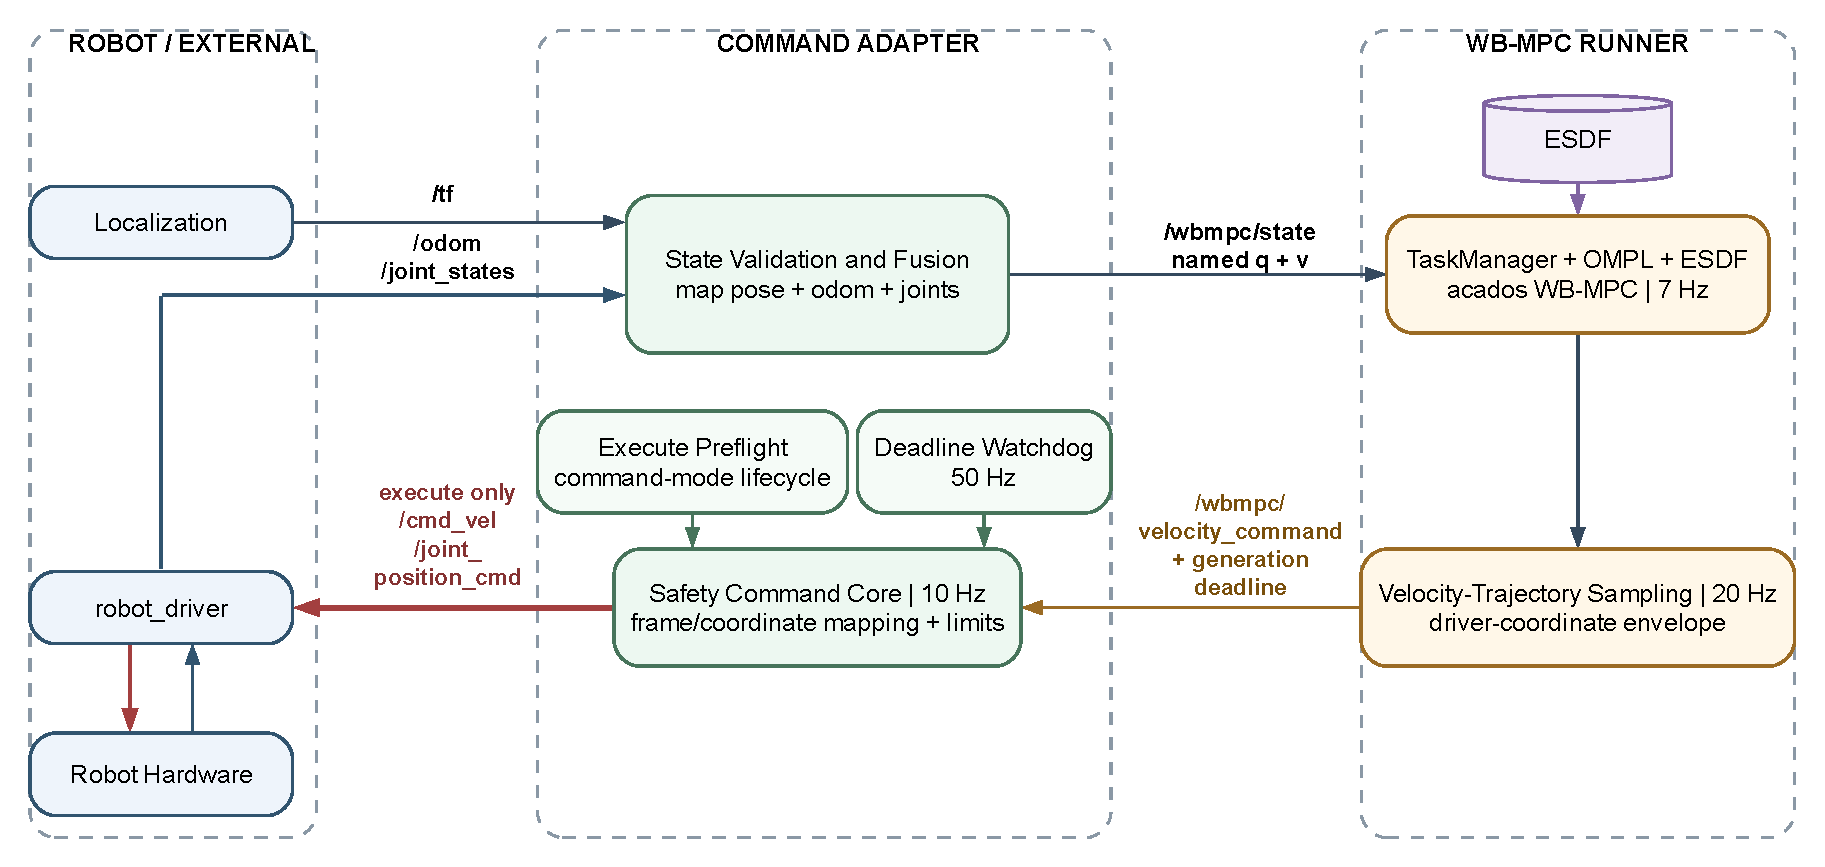
\includegraphics[width=\textwidth]{figures/ros2_node_topic_graph.pdf}
  \caption{Platform-abstract ROS~2 nodes and data flow for real-robot execution.
  The upper path carries feedback into WB-MPC, and the lower path returns the
  deadline-stamped command envelope.  Red hardware outputs exist only with
  \texttt{execute=true}; diagnostic topics and driver-mode service calls are
  omitted for legibility.}
  \label{fig:ros2-graph}
\end{figure*}

\subsection{Task-Conditioned Reference Generation}

The task manager maintains an ordered sequence of base and end-effector tasks
and exposes one active task type
$\tau\in\{\mathrm{base},\mathrm{EE}\}$ to the controller.  For a base task,
the geometric path is planned in $SE(2)$ with the RRT* implementation provided
by OMPL~\cite{sucan2012ompl,karaman2011sampling}.  The planner uses the ESDF
state-validity callback to reject configurations that violate the configured
footprint clearance, and RRT* rewires the sampling tree to reduce path cost.
For an end-effector task, the current profile uses OMPL's RRTConnect planner in
the bounded Cartesian workspace.  After path simplification, let
$\vect{\gamma}_{\tau}(s)$ denote the resulting geometric path parameterized by
progress $s$.  The reference horizon is generated from the measured path
progress $s_0$ as
\begin{align}
s_k&=\operatorname{clip}(s_0+v_{\tau}k\Delta t,0,s_{\mathrm{end}}),\nonumber\\
\vect{r}_k&=\vect{\gamma}_{\tau}(s_k),\qquad k=0,\ldots,N,
\label{eq:reference-horizon}
\end{align}
where $v_{\tau}$ is the nominal progress rate.  Thus $\vect{r}_0$ is the
current desired reference, and the remaining samples populate the MPC
prediction horizon.  A waypoint task is the constant-path special case.

The task type selects the active residual blocks in
Eq.~\eqref{eq:tracking-cost}.  A base task activates $SE(2)$ pose and base
velocity tracking and can tighten the preferred arm extension.  An
end-effector task activates Cartesian position and, when requested,
orientation and velocity tracking while allowing the optimizer to coordinate
the mobile base and manipulator through whole-body optimal control.  Residual
masks set irrelevant coordinates to zero weight.  Once the active task remains
within its configured position and orientation tolerances for the hold period,
the manager advances to the next task.
\section{System Implementation}

This section describes the execution framework and adaptation strategy
developed for real-robot deployment.

\subsection{ROS~2 Nodes and Topic Topology}

Figure~\ref{fig:ros2-graph} abstracts the real-robot execution path into a
driver, a command adapter, and a WB-MPC runner.  The
\texttt{robot\_command\_adapter} is the only application node connected to the
robot driver.  It subscribes to odometry, joint feedback, the global-to-base
transform, and the driver mode and safety states.  Valid temporally aligned
base and joint samples are combined into a named
\texttt{sensor\_msgs/JointState} on
\texttt{/wbmpc/state}.  Positions and velocities use the controller ordering,
and the header stamp and frame identify the source time and global frame used
by the controller.

The \texttt{wbmpc\_runner} subscribes to this normalized state interface.  It
owns the task manager, OMPL planners, and WB-MPC instance; the ESDF supplies
queries to both planning and control.  A worker thread starts planning and
optimization at 7~Hz so that state callbacks and the command publisher do not
block on a solve.  A separate 20-Hz timer samples the most recent valid
velocity trajectory, converts it to the driver's coordinate representation,
and publishes \texttt{/wbmpc/velocity\_command}.  The serialized envelope
contains the velocity vector, solver generation, validity flag, source-state
stamp, plan origin, and an absolute monotonic validity deadline.  The runner
and adapter publish JSON status records on \texttt{/wbmpc/status} and
\texttt{/robot\_command\_adapter/status} for logging and diagnosis.

The adapter consumes the envelope and, in execute mode, publishes base velocity
on \texttt{/cmd\_vel} and a position-oriented joint command on
\texttt{/joint\_position\_cmd} at 10~Hz. Consequently, the optimizer never owns a
driver topic directly, and all feedback validation, command conversion,
deadline enforcement, and driver-mode service calls remain at one ROS~2
boundary.

\begin{figure*}[!t]
  \centering
  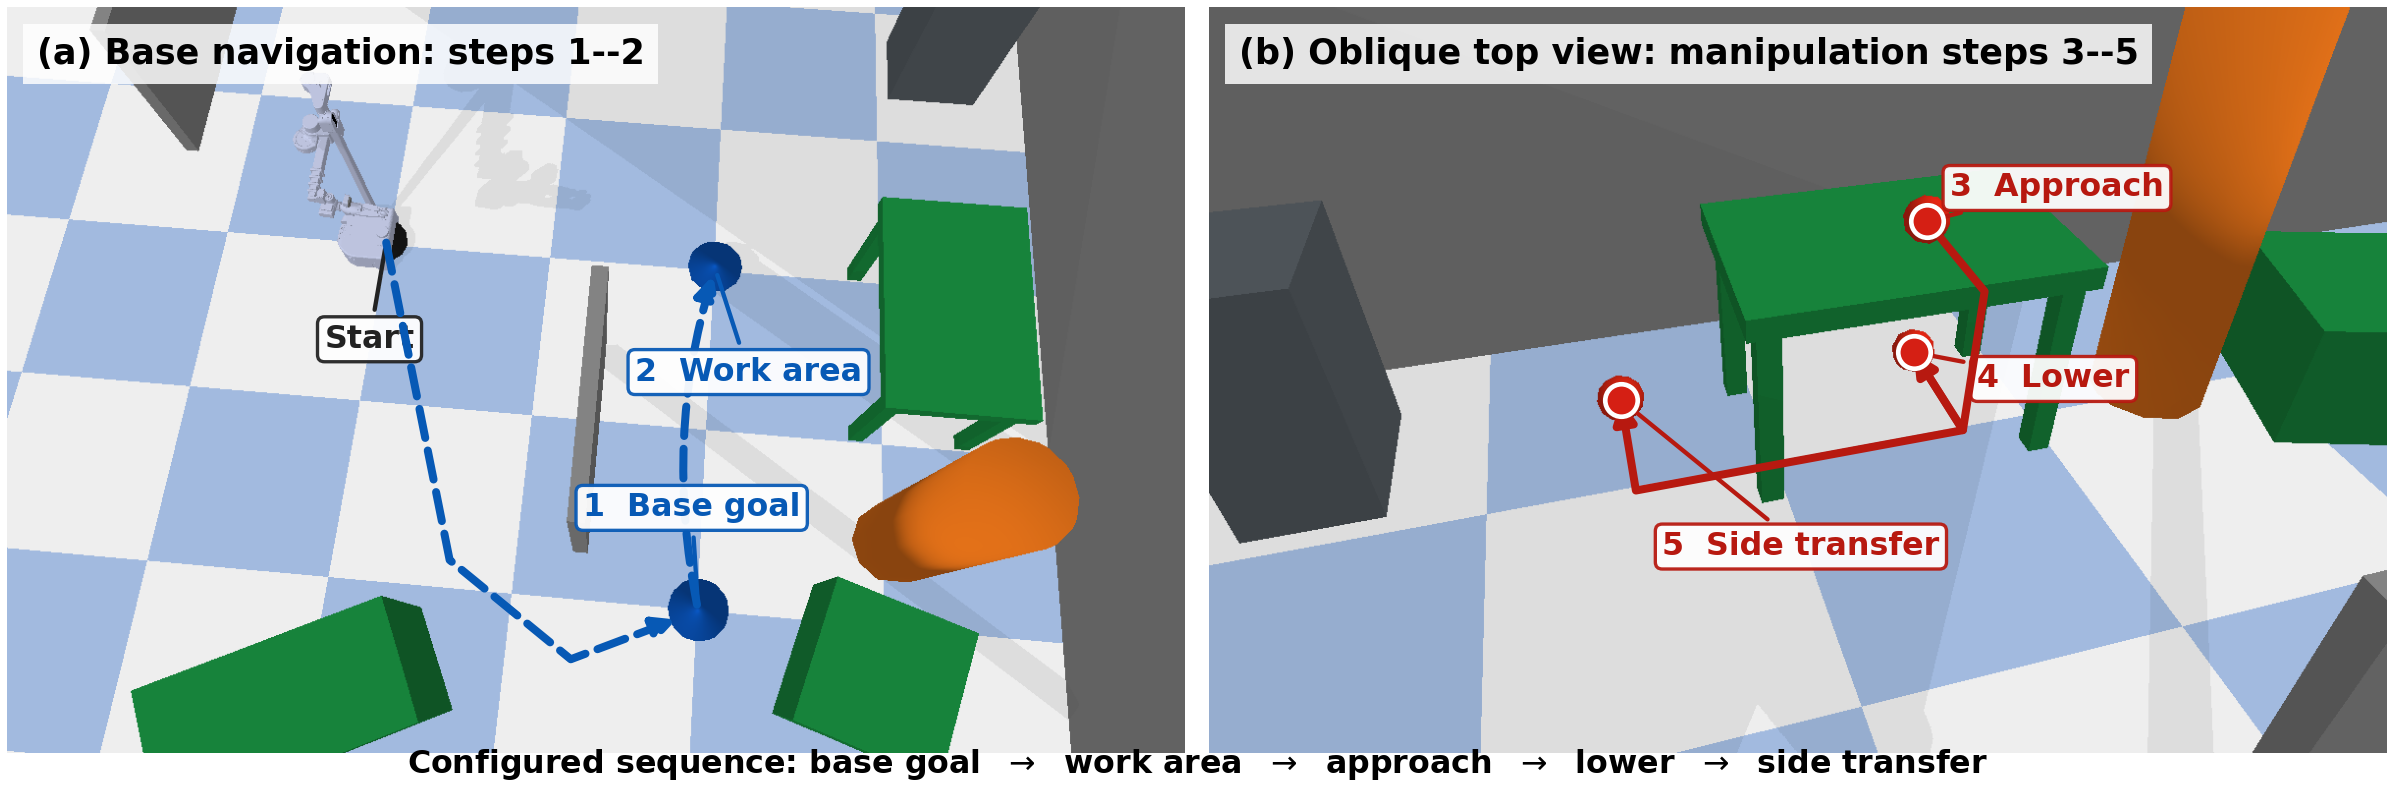
\includegraphics[width=0.96\textwidth]{figures/simulation_scenes.png}
  \caption{Complete task specified by the
  \texttt{stretch\_esdf\_offline\_ompl\_wbmpc} profile.  (a) The mobile base
  moves from its initial pose to an intermediate goal and then to the work
  area.  (b) An elevated oblique view, with the robot omitted for clarity,
  shows the end effector approaching above the work surface, reaching
  downward, and transferring laterally.  The red polylines depict a schematic
  task-space trajectory that exits the table footprint before changing height
  or moving laterally; they are not measured paths.  Numbering indicates
  execution order.}
  \label{fig:simulation-scenes}
\end{figure*}

\subsection{Forward Prediction and Deadline Hold}

In simulation, the solver and simulator run sequentially in a blocking loop,
so the simulated robot state does not evolve while the optimization is in
progress.  In real-robot deployment, however, the solver runs concurrently
with the continuously moving robot, making compensation for this motion
necessary.

The initial state used by the MPC is measured before optimization and does not
account for the robot's motion during computation.  Consequently, by the time
the optimized command reaches the robot, it is based on an outdated state.  The
runner can compensate by advancing the measured state over
\begin{equation}
\Delta t_{\mathrm{pred}}
 = a_{\mathrm{state}}+\hat{t}_{\mathrm{solve}}+t_{\mathrm{act}},
\label{eq:forward-prediction-time}
\end{equation}
where $a_{\mathrm{state}}$ is the source age of the synchronized feedback,
$\hat{t}_{\mathrm{solve}}$ is an online estimate of planning and optimization
time, and $t_{\mathrm{act}}$ is the configured dispatch and actuation latency.
After each successful cycle, the computation-time estimate is updated as
\begin{equation}
\hat{t}_{\mathrm{solve}}^{+}
=\operatorname{clip}\!\left((1-\alpha)\hat{t}_{\mathrm{solve}}
+\alpha t_{\mathrm{solve}},t_{\min},t_{\max}\right).
\label{eq:solver-time-adaptation}
\end{equation}
where $t_{\mathrm{solve}}$ is the solve time measured in the current cycle,
$\hat{t}_{\mathrm{solve}}$ is its estimate before the update, and the superscript
$+$ denotes the updated estimate.  The adaptation factor $\alpha\in[0,1]$
weights the latest measurement, while $t_{\min}$ and $t_{\max}$ bound the
updated estimate.  The current configuration sets $\alpha=0.10$, initializes
the estimate at 60~ms, clips it to $[20,120]$~ms, adds 50~ms actuation latency,
and rejects a prediction interval above 300~ms.

The initial condition imposed on the MPC is therefore
\begin{align}
\vect{x}_{0}^{\mathrm{MPC}}
&=\Phi_{\Delta t_{\mathrm{pred}}}
 \!\left(\vect{x}_{\mathrm{meas}},\vect{u}_{\mathrm{last}}\right),
\label{eq:mpc-predicted-initial-state}\\
\vect{x}_{\mathrm{meas}}
&=\begin{bmatrix}\vect{q}_{\mathrm{meas}}^{\top}&
\vect{v}_{\mathrm{meas}}^{\top}\end{bmatrix}^{\!\top}.
\nonumber
\end{align}
where $\vect{u}_{\mathrm{last}}$ is the most recently published acceleration and
$\Phi_{\tau}$ denotes propagation over duration $\tau$ using the same discrete
robot dynamics and state/input bounds as the OCP.  Without forward prediction,
$\vect{x}_{0}^{\mathrm{MPC}}=\vect{x}_{\mathrm{meas}}$.  The controller plans and
solves from this initial state and the corresponding future task time.

Command validity is bounded independently of solver termination.  The deadline
of each optimization cycle also limits the lifetime of the active command.  If
no replacement is available before this deadline, the runner invalidates the
active plan and issues a zero-velocity envelope.  A late solution can be
admitted under the configured policy, but its time origin and validity interval
are reset to its completion time; an expired command interval is never revived.

The hardware adapter independently checks the envelope deadline using a
monotonic clock.  This check ensures that a timeout produces zero base velocity
and an arm position hold even if the optimization thread stalls.  A fresh valid
command automatically releases this recoverable hold.  In contrast, violations
of state integrity, command mapping, device mode, or command ownership trigger a
latched stop that requires a restart and new preflight before execution can
resume.

\section{Experimental Evaluation}

\subsection{Experimental Setup and Metrics}

We evaluate whether the same planning and control pipeline can be specialized
to mobile manipulators with different dimensions and base kinematics.  The
framework was evaluated in PyBullet sim environment using both Stretch and mobile-UR10
configurations.  The experiment runner, task sequencing, ESDF construction,
MPC implementation, and 30-ms simulation step were held fixed across the two
platform configurations.
Only the robot-specific model, collision geometry, and controller parameters
defined by each platform profile were changed.  Consequently, the comparison
tests cross-platform execution of the framework rather than the relative
quality of the two robots or their independently tuned controllers.

The evaluated specializations are summarized in
Table~\ref{tab:platform-models}.  Stretch combines an eight-coordinate model
with the nonholonomic constraint in~\eqref{eq:no-slip}; the mobile UR10 uses a
nine-coordinate model and an omnidirectional base.  Their collision models
also differ substantially, with 34 and 93 spheres, respectively.  These
differences exercise distinct dynamics and geometry branches while preserving
the surrounding software and experimental protocol.

Figure~\ref{fig:simulation-scenes} illustrates the complete composite task in
the Stretch profile.  The robot first visits two base goals to enter the work
area, then executes an approach, vertical reach, and lateral transfer with the
end effector.  Separating the navigation and manipulation views keeps all five
configured targets visible while preserving their spatial relationship to the
same simulated workspace.

\begin{table}[t]
  \caption{Evaluated Specializations of the Shared Framework}
  \label{tab:platform-models}
  \centering
  \small
  \begin{tabular*}{\columnwidth}{@{\extracolsep{\fill}}lcc@{}}
    \toprule
    Property & Stretch & Mobile UR10 \\
    \midrule
    Optimized coordinates & 8 & 9 \\
    Arm coordinates $n_a$ & 5 & 6 \\
    Base model & nonholonomic & holonomic \\
    State dimension $n_x$ & 16 & 18 \\
    Collision spheres & 34 & 93 \\
    Extra ESDF distance & 0.07 m & 0.10 m \\
    \bottomrule
  \end{tabular*}
\end{table}

Tracking is evaluated only over samples for which the corresponding reference
is active.  For a position sequence $\vect{p}_k$ with active-reference index
set $\mathcal{I}$, we report
\begin{equation}
e_{\mathrm{RMSE}}=
\sqrt{\frac{1}{|\mathcal{I}|}\sum_{k\in\mathcal{I}}
\left\|\vect{p}_k-\vect{p}^{\mathrm{ref}}_k\right\|_2^2}.
\label{eq:position-rmse}
\end{equation}
Base-yaw RMSE is defined analogously after wrapping each angular error to
$[-\pi,\pi]$.  The final task-target error measures distance to the terminal
goal, and is therefore distinct from error to the final sample of a
time-varying reference.  Collision performance is characterized by the
minimum surface clearance, $d-r$, over all queried sphere centers, and by the
minimum safety margin, $d-r-d_{\mathrm{safe}}$.

Runtime measurements enclose the complete controller call, including
parameter construction, ESDF linearization, optimization, and diagnostics.
We additionally report solver outcomes, fallback activations, and the fraction
of calls exceeding 120~ms.  All timing results
were obtained on an Intel Core i9-14900HX.

\begin{figure*}[!t]
  \centering
  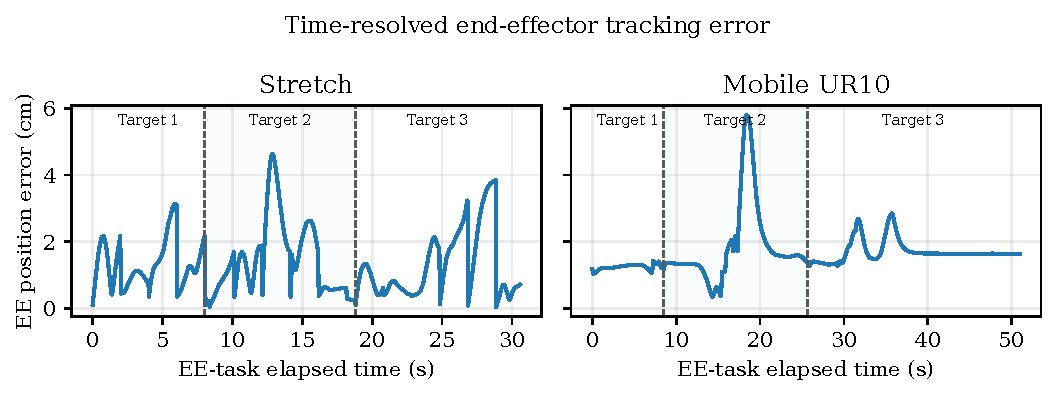
\includegraphics[width=0.92\textwidth]{figures/platform_tracking.pdf}
\caption{Euclidean EE reference-error histories for both configurations.
Time is measured from the first active EE-reference sample in each
evaluation, and both panels use the same vertical scale. Dashed lines mark
transitions between T1 (Approach), T2 (Reach Low), and T3 (Reach Side).}
  \label{fig:platform-tracking}
\end{figure*}

\begin{table}[t]
  \caption{Simulation Results for Two Robot Configurations}
  \label{tab:results}
  \centering
  \small
  \begin{tabular*}{\columnwidth}{@{\extracolsep{\fill}}lrr@{}}
    \toprule
    Metric & Stretch & Mobile UR10 \\
    \midrule
    Base position RMSE & 20.5 mm & 14.1 mm \\
    Base yaw RMSE & 6.55 mrad & 3.31 mrad \\
    EE position RMSE & 16.6 mm & 18.5 mm \\
    Minimum surface clearance & 73.2 mm & 101.5 mm \\
    Minimum safety margin & 3.22 mm & 1.47 mm \\
    Controller mean / P95 & 81.4 / 141.0 ms & 71.4 / 80.4 ms \\
    Controller maximum & 785.3 ms & 799.3 ms \\
    Calls above 120 ms & 7.50\% & 1.05\% \\
    Solver status 0 / 2 & 1296 / 38 & 1998 / 2 \\
    \bottomrule
  \end{tabular*}
\end{table}

\subsection{Cross-Platform Tracking}

Across both configurations, the shared controller maintained centimeter-level
tracking despite differences in base mobility, arm dimension, collision
geometry, and tool-frame definition.  Base-position RMSE ranged from 14.1 to
20.5~mm, base-yaw RMSE from 3.31 to 6.55~mrad, and EE-position RMSE from 16.6
to 18.5~mm.  These results indicate that the same optimization and execution
pipeline can accommodate distinct kinematic structures without embedding a
single platform's motion model in the common planner.  Platform-specific
constraints, such as the nonholonomic dynamics in
Equation~\eqref{eq:no-slip}, enter through the configured model.

The comparison is intended as a portability test rather than a ranking of the
two robots.  Each configuration instantiates its own state dimension, base
dynamics, arm coordinates, collision representation, and tracking weights,
while retaining the same controller structure and execution path.  Variations
in completion and terminal error therefore reflect the combined effects of
platform dynamics, scenario duration, reference evolution, and tuning; they
should not be attributed to morphology alone.  The aggregate results are
summarized in Table~\ref{tab:results}.

Similar aggregate RMSE values can nevertheless mask platform-dependent error
structure.  Axis-wise EE errors differ across the two configurations, with the
largest contribution occurring on different axes and with different temporal
profiles.  For this reason, cross-platform evaluation should report both
aggregate tracking metrics and time-resolved errors.
Figure~\ref{fig:platform-tracking} provides these complementary views.

\subsection{ESDF Clearance}

All ESDF queries were valid on both robots.  Minimum executed-state surface clearance,
defined as distance minus sphere radius, was 73.2~mm for Stretch and 101.5~mm
for the mobile UR10.  After subtracting their separately configured 70- and
100-mm safety distances, the minimum executed-state margins were positive but
small: 3.22 and 1.47~mm.  The pre-optimization warm-start horizon reached
$-24.5$ and $-83.9$~mm, respectively.  These negative warm-start margins were
not executed-state collisions.  During re-optimization, the ESDF collision
cost further safeguarded execution by steering the candidate trajectory away
from obstacles.  If acados terminated at its SQP-iteration limit (status 2), a
separate post-solve acceptance check examined the resulting trajectory before
it could be issued: all state and control entries had to be finite, every ESDF
query for every collision sphere and shooting node had to be valid, and the
minimum horizon margin, $d-r-d_{\mathrm{safe}}$, had to be no smaller than the
configured 0-mm threshold.  Failure of any check caused a zero-velocity
fallback.  Thus, the negative-margin warm starts above were not issued as
commands.  The same post-solve horizon margins should in future be logged for
every solver outcome, rather than only when status 2 triggers this check.

\begin{figure*}[!t]
  \centering
  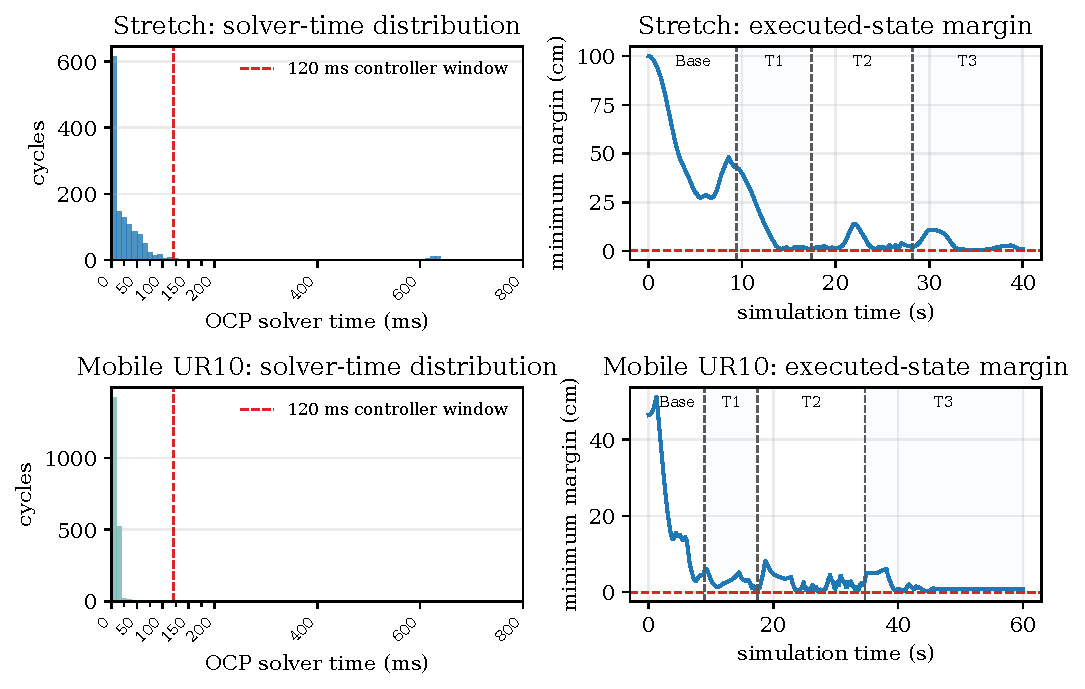
\includegraphics[width=0.92\textwidth]{figures/platform_timing_clearance.pdf}
  \caption{OCP solver-time distributions and minimum executed-state ESDF
  margins for Stretch (top) and mobile UR10 (bottom).  Solver-time histograms
  use 10-ms bins, with finer ticks over 0--200~ms.  In the margin panels,
  vertical dashed lines separate the base-motion phase from T1 (Approach), T2
  (Reach Low), and T3 (Reach Side).  The 120-ms line shows the shared controller
  validity-window reference; the zero-margin line denotes each profile's own
  configured collision boundary.}
  \label{fig:platform-timing-clearance}
\end{figure*}

\subsection{Solver and Runtime Timing}

Complete controller time averaged 81.4~ms for Stretch and 71.4~ms for the
mobile UR10.  Their P95 values were 141.0 and 80.4~ms, but isolated maxima of
785.3 and 799.3~ms show long tails on both.  The solver-status row in
Table~\ref{tab:results} uses the acados return codes: status 0 denotes
successful convergence, whereas status 2 denotes the configured SQP-iteration
limit.  The status-2 acceptance check defined above admitted all 38 such
Stretch cycles; of the mobile UR10's two status-2 cycles, one was admitted and
one produced the zero-velocity fallback.  The 93-sphere UR10 profile
spent more mean time in parameter update and ESDF linearization (51.3 and
37.4~ms) than Stretch (30.6 and 15.9~ms), yet its easier OCP solves averaged
8.74 rather than 41.6~ms.  This decomposition shows that robot geometry and
optimization difficulty affect different runtime components; configurability
does not imply platform-independent timing.

Table~\ref{tab:runtime-breakdown} gives the distribution and solver-iteration
details.  Parameter update includes all shooting-node parameters, and ESDF
linearization is nested within that work; the rows must therefore not be
summed as independent totals.  The UR10's larger sphere set increases the
largely deterministic parameter cost, whereas Stretch's difficult SQP cycles
dominate its upper tail.  In particular, the median-to-P99 jump from 53.6 to
700.6~ms for Stretch is much larger than the mobile UR10's 68.6 to 120.3~ms.

\begin{table}[t]
  \caption{Runtime and Solver Breakdown}
  \label{tab:runtime-breakdown}
  \centering
  \small
  \begin{tabular*}{\columnwidth}{@{\extracolsep{\fill}}lrr@{}}
    \toprule
    Metric & Stretch & Mobile UR10 \\
    \midrule
    Controller median / P99 (ms) & 53.6 / 700.6 & 68.6 / 120.3 \\
    OCP solve mean / P95 (ms) & 41.6 / 100.2 & 8.74 / 16.0 \\
    Parameter update mean (ms) & 30.6 & 51.3 \\
    ESDF linearization mean (ms) & 15.9 & 37.4 \\
    SQP iterations mean / P95 & 32.0 / 77.7 & 5.15 / 10.0 \\
    SQP iterations maximum & 500 & 500 \\
    Accepted nonzero status & 38 & 1 \\
    Zero-velocity fallback & 0 & 1 \\
    \bottomrule
  \end{tabular*}
\end{table}

Figure~\ref{fig:platform-timing-clearance} shows why both central tendency and
tails are necessary.  It compares the OCP solver-time distribution with the
executed-state collision-margin history for each robot.  The margin histories
are divided into the base-motion phase and three end-effector task phases.  No
causal relationship should be inferred directly from this plot: solver
difficulty depends on tracking, active costs, bounds, and local ESDF geometry
simultaneously.

\subsection{Real-Robot Deployment}

The control framework was successfully deployed on the physical Stretch
platform.  Spectacular AI SLAM localizes the base in the shared map frame.  The
environment is reconstructed with nvblox, and its ESDF is exported offline and
loaded by the controller~\cite{millane2023nvblox}.  Robot state, Spectacular AI
localization, and static ESDF queries are then combined to optimize and execute
whole-body commands through the Stretch interface, demonstrating the complete
mapping--localization--control pipeline on real hardware.  Videos are available
in the
\href{https://drive.google.com/drive/folders/1bsqAc2rYdHWyNgyATlZ9J\_RCnpOuP5xE?usp=drive\_link}{online demo folder}.

\section{Discussion}

The two evaluated configurations provide executable evidence that the central planning and
control framework is not specific to Stretch.  Without changing the common
experiment runner or MPC class, it instantiated different state dimensions,
arm chains, tool frames, collision-sphere sets, clearances, and base dynamics.
Both configurations tracked moving references to centimeter accuracy and used
base motion during manipulation.  This supports adaptability to the two tested
mobile manipulators.

The framework is effective in part because planning and control provide two
complementary layers of collision avoidance.  First, OMPL uses ESDF-based state
validity checks to generate a collision-checked reference path with the
configured clearance.  This supplies the controller with a globally meaningful
route around obstacles instead of requiring a short MPC horizon to discover
one.  Second, WB-MPC evaluates the ESDF collision cost over the predicted
whole-body trajectory and can modify the local motion while enforcing the
robot dynamics and tracking the reference.  The planner therefore protects the
geometric path, while the MPC provides additional protection against clearance
loss during execution.  Because both layers query the same ESDF, their
collision reasoning remains geometrically consistent.  The positive
executed-state margins observed for both robots support the effectiveness of
this two-layer design in the evaluated scenarios.

The runtime decomposition also highlights the role of base mobility in OCP
difficulty.  Although the mobile UR10 uses the larger collision-sphere set and
spends more time on parameter updates and ESDF linearization, its OCP solves
required only 8.74~ms and 5.15 SQP iterations on average, compared with
41.6~ms and 32.0 iterations for Stretch.  The UR10's holonomic base permits
independent planar translation, whereas Stretch's nonholonomic constraint
couples translational motion to its heading.  The resulting increase in
instantaneously feasible correction directions can make simultaneous tracking
and collision avoidance easier to solve.  The results therefore suggest that
base mobility can affect optimization difficulty more strongly than the
collision-model size alone.

The positive 3.22- and 1.47-mm minimum margins show that both robots respected
their configured collision boundaries throughout the evaluated trajectories.
Together with the tracking results, this demonstrates simultaneous task
execution and modeled whole-body clearance for two distinct mobile-manipulator
configurations.  The real Stretch deployment uses a static ESDF exported from
nvblox and aligned with Spectacular AI SLAM, providing a consistent
geometric reference across mapping, planning, and control.  As expected for a
precomputed map, changes made after export are outside its representation;
online updates and platform safety mechanisms can complement this map when
operating in dynamic environments.

\section{Conclusion}

This work demonstrates that heterogeneous mobile manipulators can share a
configurable ESDF-aware planning and whole-body control pipeline.  OMPL provides
a globally collision-checked reference, while the WB-MPC collision cost adds
local clearance protection during execution.  The same implementation achieved
centimeter-level tracking and positive executed-state margins on nonholonomic
Stretch and holonomic mobile-UR10 models.  The UR10 OCP was easier to solve
despite its larger collision model, showing the importance of base mobility to
optimization difficulty.  Deployment on the physical Stretch with Spectacular
AI SLAM, an offline nvblox ESDF, and the guarded ROS~2 interface confirms that
the architecture extends beyond simulation.

\section{Future Work}

Future work will first investigate an object-centric ESDF constructed from
semantic object detections, estimated poses, and geometric models.  Compared
with an ESDF built directly from RGB-D measurements, this representation could
provide more stable collision boundaries in the presence of depth noise and
missing measurements.  A second direction is to close the loop between perception,
mapping, navigation, and manipulation.  A shared scene representation would
allow new observations to update the map, navigation to position the mobile
base, and WB-MPC to complete manipulation while triggering replanning when the
scene changes.

\appendix

\noindent Code repository:\\
\url{https://github.com/stateirving/mobile_manipulation}

\noindent Demonstration videos:\\
\url{https://drive.google.com/drive/folders/1bsqAc2rYdHWyNgyATlZ9J_RCnpOuP5xE?usp=drive_link}

\balance
\bibliographystyle{IEEEtran}
\bibliography{references}

\end{document}
